
\section{Einführung in den CUBE ProjectAssistant} % Major section
% Example citation \cite{Figueredo:2009dg}. (Literaturangabe; Literaturliste)

In dieser Anleitung wird die Kurzform CUBE PA verwendet.

\subsection{Wofür dient der CUBE PA?} % Sub-section

Der CUBE PA ist ein Hilfsmittel für das Projektmanagement. Als Datenbankapplikation mit webbasiertem Zugriff lässt er sich an jedem Ort mit Internetverbindung zu jeder Zeit nutzen. Er unterstützt für das Projektmanagement typische Workflows wie das Sitzungswesen, Dokumentenablage, Anforderungs- und Mängelmanagement oder das Beschaffungswesen und macht alle Informationen, die im Lauf der Projektmanagementarbeit anfallen, überall und jederzeit verfügbar.

\subsection{Wer soll den CUBE PA benutzen?} % Sub-section

Der CUBE PA ist vor allem für Projekte nützlich, die einige der folgenden Merkmale aufweisen:

% \begin{itemize} % - Zu grosser Abstand verwendet
% 	\item xy
% \end{itemize}
	
\begin{compactitem}
	\item Etliche involvierte Parteien, Firmen, Organisationen
	\item Die Akteure sind an verschiedenen Arbeitsorten tätig
	\item Komplexe Struktur mit vielen Teilprojekten
	\item Längere Dauer
	\item Grosse Mengen an Sitzungen, Dokumenten, Pendenzen, Beschaffungen etc.
	\item Zeitverschiebung zwischen den Akteuren
	\item Bedarf nach flexibler Arbeitsmöglichkeit ausser Haus, im Zug, Tag und Nacht etc.
\end{compactitem}	
		
\ \\
Ist ein Projekt zur Verwendung des CUBE PA auserkoren, ist es von zentraler Bedeutung, dass möglichst alle in das Projektmanagement involvierten Personen den CUBE PA benutzen. Dies betrifft sowohl die Entscheidungsträger als auch ihre Assistenten. Nur so kann der maximale Nutzen aus dem Anfangsaufwand für das Aufsetzen des CUBE PA erreicht werden.
	
\subsection{Gliederung des CUBE PA} % Sub-section

Der CUBE PA ist in die unten beschriebenen Bereiche gegliedert, die einem Punkt im Menü entsprechen. Weitere Module werden in Abhängigkeit von Projekten oder sonstigen Anforderungen entwickelt. Nachfolgend wird jeder Bereich kurz beschrieben, um dem Leser einen Anhaltspunkt zum Verwendungszweck und zum Entwicklungsstand zu geben. Für jeden Bereich ist weiter unten in einem eigenen Kapitel beschrieben, wie er benutzt wird.

\pagebreak
\subsubsection{Das CUBE PA-Menü} % Sub-sub-section

\setlength{\abovecaptionskip}{0pt}

\begin{wrapfigure}[16]{l}{7cm}   % [x] Wie manche Zeile soll sich um die Grafik "brechen"
  \vspace{-25pt}      % Grundwert war 20; mit 30 schön oben beim Text ausgerichtet
  \begin{center}
    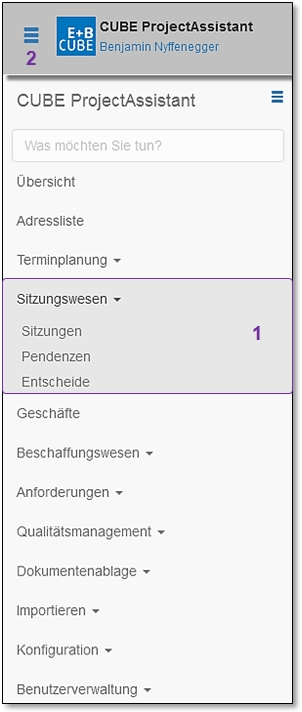
\includegraphics[height=150mm]{../chapters/01_Einfuehrung/pictures/1-3-1_Menuuebersicht_oSitzungswesen.jpg}
  \end{center}
  \vspace{-20pt}
  \caption{Das Menü}
  \vspace{-10pt}
\end{wrapfigure}
Die verschiedenen Bereiche des CUBE PA können Sie jederzeit über das Menü erreichen. Je nach Bereich können Sie zwischen verschiedenen Unterkategorien auswählen. Klicken Sie dazu auf das gewünschte Thema. Befinden sich darin weitere Unterthemen werden diese angezeigt. Unter „Sitzungswesen“ \col{(1)} werden die drei Unterkategorien „Sitzungen“, „Pendenzen“ und „Entscheide“ aufgelistet. Durch Mausklick auf die gewünschte Unterkategorie wird diese geöffnet. Mit erneutem Klick auf den Themenbereich (Sitzungsbereich), klappen die Unterthemen wieder ein. 

\vspace{\baselineskip}

Mit Klick auf das Menü-Icon \col{(2)} können Sie das Menü ein- und ausblenden. So steht Ihnen eine grössere Arbeitsfläche zur Verfügung.

\vspace{6.5cm}  

\textbf{Angepasstes Menü}

\begin{wrapfigure}[7]{r}{5.5cm}
\vspace{-35pt}
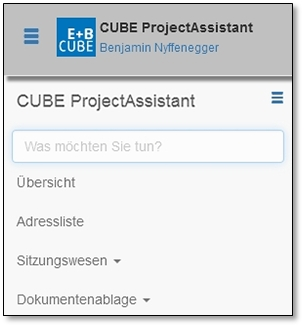
\includegraphics[height=60mm]{../chapters/01_Einfuehrung/pictures/1-3-1_MenuAngepasst.jpg}
\caption{Angepasstes Menü}
\end{wrapfigure}

Abhängig von den Berechtigungen, welche einem Nutzer gegeben werden, kann sich das Menü in der Vielfalt / den sichtbaren Menüpunkten zu den Printscreens in dieser Anleitung wie auch zu anderen Benutzern (andere Rollen, z.B. Administrator) unterscheiden. In der vorliegenden Anleitung werden jeweils sämtliche Menüpunkte abgebildet.

\subsubsection{Übersicht}
\label{bkm:Ref132000001}
Die persönliche Übersicht erscheint als erstes, wenn Sie sich beim CUBE PA angemeldet haben. Sie gibt einen schnellen Überblick über Sachverhalte, die Sie direkt betreffen.

\begin{figure}[H] % Example image
\center{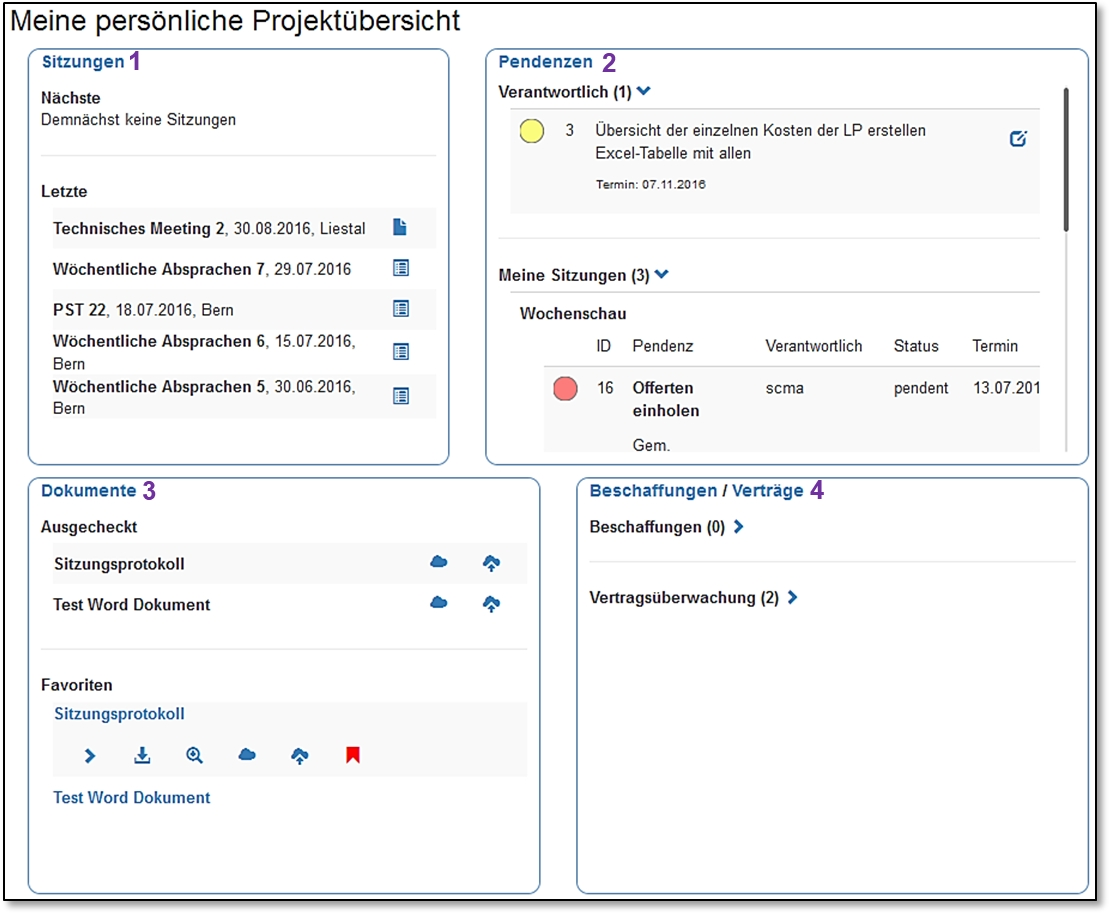
\includegraphics[width=1\linewidth]{../chapters/01_Einfuehrung/pictures/1-3-2_persUebersicht.jpg}}
\caption{Meine persönliche Projektübersicht}
% \label{fig:speciation}
\end{figure}

Oben links erscheinen die aktuellen Sitzungen \col{(1)}. Unter „Nächste“ erscheinen demnächst stattfindende Sitzungen mit Ihrer Beteiligung. Sie haben die Möglichkeit eine Sitzungseinladung zu bearbeiten oder für den Versand als pdf zu speichern. Unter „Letzte“ werden Sitzungen dargestellt, die kürzlich stattgefunden haben. Mit einem Klick können Sie das Protokoll öffnen. Ist noch kein definitives Protokoll vorhanden, können Sie dieses noch bearbeiten. Wenn Sie auf den blauen Titel „Sitzungen“ \col{(1)} klicken, wechseln Sie direkt in den Unterpunkt „Sitzungen“ der Rubrik „Sitzungswesen“.

\vspace{\baselineskip}

Oben rechts erscheinen die Pendenzen \col{(2)}, für die Sie verantwortlich oder bei deren Erledigung Sie beteiligt sind (Mitarbeit). Mit einem Klick können Sie eine Pendenz bearbeiten. Die entsprechende Maske wird geöffnet. Wenn Sie auf den blauen Titel „Pendenzen“ \col{(4)} klicken, wechseln Sie direkt in den Unterpunkt „Pendenzen“ der Rubrik „Sitzungswesen“. Siehe Kapitel 5.4 für das Erstellen und 5.5 für die Bearbeitung von Pendenzen.

\vspace{\baselineskip}

Links unten erscheinen für Sie relevante Dokumente \col{(3)}. Unter „Ausgecheckt“ werden die von ihnen ausgecheckten Dokumente angezeigt. Sie haben die Möglichkeit ein ausgechecktes Dokument von hier aus zu öffnen oder es wieder einzuchecken. \\

Unter „Favoriten“ werden diejenigen Dokumente aufgelistet, die von Ihnen als persönliche Favoriten markiert wurden. Mit Klick auf den blauen Dokumententitel erscheinen die möglichen Optionen: Sie haben die Möglichkeit ein favorisiertes Dokument herunterzuladen, Details anzuschauen, den Eintrag zu ändern oder das Dokument auszuchecken, damit Sie es bearbeiten können und es während dieser Zeit für andere gesperrt ist. Ebenso können Sie ein favorisiertes Dokument in der Vorschau betrachten. Falls Sie ein Dokument nicht mehr als Favorit benötigen, klicken Sie auf das rote Flag-Symbol und der Eintrag verschwindet nach einem Aktualisieren der Ansicht oder erneutem Klick auf die 'Übersicht'. Mit erneutem Klick auf den Dokumententitel werden die Optionen zur besseren Übersicht wieder ausgeblendet. Wenn Sie auf den blauen Titel „Dokumente“ \col{(3)} klicken, wechseln Sie direkt in den Unterpunkt „Dokumente“ der Rubrik „Dokumentenablage“.

\vspace{\baselineskip}

% Text, welcher bis zur Grafik reichen soll, ist unmittelbar an Grafikeinbettung 
% zu schreiben, dann kommt Grafikeinbettung, dann Text, welcher Grafik umschliesst.

\begin{wrapfigure}{r}{0.5\textwidth}
  \vspace{-20pt}
  \begin{center}
    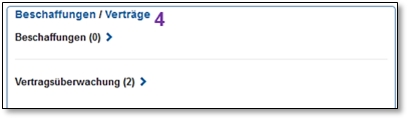
\includegraphics[width=0.5\textwidth]{../chapters/01_Einfuehrung/pictures/1-3-2_persUebersichtBeschaffung.jpg}
  \end{center}
  \vspace{-20pt}
%  \caption{Persönliche Übersicht}
  \vspace{-10pt}
\end{wrapfigure}
Rechts unten erscheinen die Beschaffungen \col{(4)} und Vertragsüberwachungen, an denen Sie beteiligt sind, und bei denen eine Aktion von Ihnen erwartet wird. In Klammern sehen Sie bei wie vielen Einträgen Sie involviert sind. Klicken Sie auf das horizontale Pfeilsymbol, um sich die Beschaffungen oder einer Vertragsüberwachung anzeigen zu lassen. Von hier aus können Sie mit Klick auf das Lupensymbol neben einer Beschaffung oder eine Vertragsüberwachung direkt in die entsprechende Beschaffung wechseln und diese dann bearbeiten. Je nach Stand der Beschaffung kann es aber sinnvoller sein via Menü und dem Punkt Beschaffungswesen und den dort vorhandenen Unterpunkte an die richtige Bearbeitungsmöglichkeit zu gelangen. Siehe Kapitel 7 über das Beschaffungswesen. Wenn Sie auf die blauen Titel „Beschaffungen“ resp. „Verträge“ \col{(4)} klicken, wechseln Sie direkt in die Unterpunkte „Beschaffungen“ resp. „Verträge“ der Rubrik „Beschaffungswesen“.

\vspace{\baselineskip}

\begin{wrapfigure}[5]{r}{0.5\textwidth}
  \vspace{-30pt}
  \begin{center}
    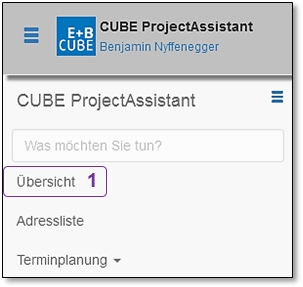
\includegraphics[width=0.4\textwidth]{../chapters/01_Einfuehrung/pictures/1-3-2_MenuepunktUebersicht.jpg}
  \end{center}
  \vspace{-20pt}
  \caption{Menü Übersicht}
  \vspace{-10pt}
\end{wrapfigure}
Wenn Sie mittels dem Menü in einen anderen Bereich wechseln, verlassen Sie die persönliche Übersicht. Um wieder dorthin zu gelangen, klicken Sie im Menü den Punkt „Übersicht“ \col{(1)}.

\pagebreak
\subsubsection{Adressliste}

In der Adressliste werden auf einfache Art und Weise sämtliche im CUBE PA erfassten Personen (Benutzer) und Firmen (Beteiligte) angezeigt. Mittels der Filterfunktion können die gesuchten Einträge rasch gefunden werden.

\subsubsection{Terminplanung}

Die Funktionalität ist derzeit rudimentär und beschränkt sich im Wesentlichen auf das Herunterladen von Dokumenten. Sie ist deshalb vorläufig nicht im Detail beschrieben. Beim 'Detailterminprogramm' handelt es sich um einen Microsoft-Project Import (xml-File), welcher dann ein Filtern und Anzeigen der eingelesenen Daten ermöglicht.

\subsubsection{Sitzungswesen}

Der CUBE PA unterstützt den vollständigen Workflow für das Einladen zu und das Protokollieren von Sitzungen, mit Ausnahme der Kalender- und Raumbuchungen, die typischerweise in Outlook erfolgen. Die für eine Sitzungseinladung erfassten Daten stehen automatisch als Grundlage für das Protokoll zur Verfügung. Dieses kann direkt im CUBE PA erfasst und von den Teilnehmern korrigiert werden. Ebenfalls steht eine Pendenz- und Entscheidverwaltung zur Verfügung.

\subsubsection{Geschäfte}

Der CUBE PA unterstützt ein einfach zu erfassendes, strukturiertes Projektjournal. Wird dieses gewissenhaft geführt, sind alle Projektbeteiligte immer und überall auf dem neuesten Stand der Dinge.

\subsubsection{Anforderungs- und Mängelmanagement}

Das 'Anforderungs- und Mängelmanagement' dient der Abnahme von Projekten. Sämtliche Mängel werden dokumentiert und mit 'Arbeitspaketen' und Pendenzen verknüpft. So haben Sie jederzeit den Überblick über eine Abnahme und wissen genau, welche Arbeiten noch erledigt oder nachgebessert werden müssen.

\subsubsection{Beschaffungswesen}

Der CUBE PA unterstützt den vollständigen Workflow einer Beschaffung, von der Offertanfrage über die Offerte und die Offertprüfung zum Vertrag. Die Verknüpfungen zwischen Offertanfrage, Offerte und Vertrag sind über ein intelligentes Nummerierungssystem einfach ersichtlich. Derzeit ist nur die Funktionalität für Beschaffungen mit einem Anbieter (freihändiges Verfahren) implementiert, die Funktionalität für Beschaffungen mit mehreren Anbietern folgt in einem nächsten Entwicklungsschritt.

\subsubsection{Qualitätsmanagement / Handbücher}

Die Funktionalität ist derzeit rudimentär und beschränkt sich im Wesentlichen auf das Herunterladen von Dokumenten. Die Funktionalität 'Handbücher' ermöglicht das vollständige Erfassen von Projekt- oder anderen Handbücher im CUBE PA.

\subsubsection{Customer Relationship Management}

Das CRM (Customer Relationship Management) ermöglicht Ihnen effizient Veranstaltungen (Anlässe, Präsentationen und Schulungen) zu koordinieren. Es unterstützt Sie bei der Einladung, dem Verwalten von Anmeldungen, Versenden von Erinnerungen und dem Erstellen von Teilnehmerlisten. Für Ihre Veranstaltung erstellen Sie über eine Webseite eine Einladung in Form eines Online-Flyers, auf welchem sich die Teilnehmer an- oder abmelden können.

\subsubsection{Dokumentenablage}

Die Dokumentenablage ermöglicht das versionierte Ablegen von Dokumenten aller Art. Die abgelegten Dokumente können mit Metadaten / Tags gekennzeichnet werden. Nebst der Möglichkeit Dokumente Ein- und Auszuchecken und direkt in den Office-Programmen zu bearbeiten (wie bei Microsoft SharePoint), können die Dokumente online betrachtet werden (Vorschaufunktion). Jedes Dokument kann einem geografischen Ort zugewiesen werden (Doppelklick direkt in die Google-Map). Der Ort kann nachträglich per Drag’n’Drop in der Karte verschoben werden. Die Dokumentenablage ermöglicht eine Übersicht über geografisch benachbarte Dokumente.

\subsubsection{Importieren}

Mittels dieser Option können Terminpläne und Geschäfte (Daten) importiert werden.

\subsubsection{Konfiguration}

Die Konfiguration dient dazu, projektspezifische Daten zu erfassen, die anschliessend in Auswahllisten erscheinen sollen. Diese Arbeit muss normalerweise nur von wenigen Personen geleistet werden und wird deshalb nur rudimentär beschrieben.

\subsubsection{Benutzerverwaltung}

In der Benutzerverwaltung werden Benutzer, Teams sowie Gruppen erfasst.

